\documentclass[a4paper,12pt]{article}

\title{Chapter 2. The Klein-Gordon Field\\
2-4. The Klein-Gordon Field in Space-Time}
\date{各種SNS\\
    X (旧 Twitter): \href{https://x.com/miya_max_study}{@miya\_max\_study}\\
    Instagram : \href{https://www.instagram.com/daily_life_of_miya/}{@daily\_life\_of\_miya}\\
    YouTube : \href{https://www.youtube.com/@miya-max-active}{@miya-max-active}
    }
\author{Max Miyazaki}

\usepackage{amsmath}
\usepackage{amssymb}
\usepackage{ascmac}
\usepackage{amsthm}
\usepackage{amsfonts}
\usepackage{enumitem}
\usepackage{color}
\usepackage[dvipdfmx]{graphicx}
\usepackage{float}
\usepackage{bm}
\usepackage{here}

\usepackage{abstract}
\usepackage{tikz}
\usetikzlibrary{shapes.geometric, arrows.meta, positioning}
\usepackage{indentfirst}
\usepackage[utf8]{inputenc}
\usepackage{fix-cm}
\usepackage{wrapfig}
\pagenumbering{arabic}
\usepackage{url}
\usepackage{xcolor}
\usepackage[most]{tcolorbox}
\usepackage{framed}
\usepackage[dvipdfmx]{hyperref}
\hypersetup{
 setpagesize=false,
 bookmarksnumbered=true,
 colorlinks=true,
 linkcolor=blue
}

% Define braket-like commands
\newcommand{\bra}[1]{\left\langle #1\right|}
\newcommand{\ket}[1]{\left|#1\right\rangle}
\newcommand{\braket}[2]{\left\langle #1\middle|#2\right\rangle}
\newcommand{\brakets}[3]{\left\langle #1\middle| #2 \middle|#3 \right\rangle}

\renewcommand{\arraystretch}{2.1}


\setlength{\textwidth}{16cm}
\setlength{\textheight}{25cm}
\setlength{\oddsidemargin}{0cm}
\setlength{\evensidemargin}{0cm}
\setlength{\topmargin}{-2cm}

\begin{document}
\maketitle

\vspace{1cm}
\begin{abstract}
    このノートはPeskin\&Schroederの``An Introduction to Quantum Field Theory''の第2章の3節をまとめたものである. 要点や個人的な追記, 計算ノート的なまとめを行っているが, それらはすべて原書の内容を出発点としている. 参考程度に使っていただきたいが, このノートは私の勉強ノートであり, そのままの内容をそのまま鵜呑みにすると間違った理解を招く可能性があることをご了承ください. ぜひ原著を手に取り, その内容をご自身で確認していただくことを推奨します. てへぺろ v$({\hat{\cdot}_\partial \hat{\cdot}})$v



\end{abstract}
    
    

\newpage

\color{blue}
\section*{概要}
\begin{itemize}
  \item Klein-Gordon場 $\phi(x)$ および共役運動量 $\pi(x)$ をHeisenberg描像で時間依存の演算子として扱う.
  \item 時間発展はHeisenberg方程式より与えられ, Klein-Gordon方程式を満たす:
  \begin{equation*}
    (\Box + m^2)\phi(x) = 0.
  \end{equation*}
  \item 場のモード展開は正・負の周波数モードからなり, それぞれ粒子の消滅・生成を意味する.
\end{itemize}

\subsection*{因果性}
\begin{itemize}
  \item 場の交換関係 $[\phi(x), \phi(y)]$ は $(x - y)^2 < 0$ のときゼロになる.
  \item これは局所場理論における因果律の要請を満たす条件である.
  \item 因果性を保つためには, 反粒子の存在が不可欠である.
\end{itemize}

\subsection*{Green関数と伝播子}
\begin{itemize}
  \item 遅延Green関数 $D_R(x - y)$ は
  \begin{equation*}
    (\Box + m^2) D_R(x - y) = -i \delta^{(4)}(x - y)
  \end{equation*}
  を満たし, 因果性を保つ解を与える.
  \item Feynman伝播関数は時間順序付きの期待値で定義される:
  \begin{equation*}
    D_F(x - y) = \langle 0 | T \phi(x) \phi(y) | 0 \rangle
  \end{equation*}
\end{itemize}

\subsection*{古典ソースによる粒子生成}
\begin{itemize}
  \item 古典外部ソース $j(x)$ を用いた方程式:
  \begin{equation*}
    (\Box + m^2)\phi(x) = j(x)
  \end{equation*}
  \item 解はGreen関数との畳み込みで表される.
  \item ソースによって生成される粒子数は,
  \begin{equation*}
    N = \int \frac{d^3p}{(2\pi)^3} \frac{|\tilde{j}(p)|^2}{2E_p}
  \end{equation*}
  で与えられる. ただし, $\tilde{j}(p)$ はフーリエ変換, $\displaystyle \tilde{j}(p) = \int d^4 y\, e^{ip \cdot y} j(y)$ である.
\end{itemize}

\color{black}
\section*{2-4. The Klein-Gordon Field in Space-Time}
前節では, Klein-Gordon 場を Schr\"{o}dinger 描像で量子化し, その理論を相対論的粒子の観点から解釈した. 本節では Heisenberg 描像に切り替え, 時間依存量や因果性の問題を議論しやすくする. その後, セクション2.1で提起された因果的伝播の問題に立ち返る. また, Feynman 則の重要な構成要素である Klein-Gordon 伝播子の表式を導出する.\par
Heisenberg 描像では, 演算子 $\phi$ および $\pi$ を次のように時間依存に定義する:
\begin{equation*}
\phi(x) = \phi(\mathbf{x}, t) = e^{iHt} \phi(\mathbf{x}) e^{-iHt}, \tag{2.43}
\end{equation*}
$\pi(x) = \pi(\mathbf{x}, t)$ も同様. Heisenberg の運動方程式は,
\begin{equation*}
i \frac{\partial}{\partial t} \mathcal{O} = [\mathcal{O}, H]. \tag{2.44}
\end{equation*}
\textcolor{blue}{※ $\mathcal{O}$ は任意の演算子で, $\phi$ や $\pi$, 粒子数演算子など, 物理的観測対象に対応するもの. }
\vskip\baselineskip
これにより, $\phi$ および $\pi$ の時間依存性が次のように計算できる:
\begin{align*}
i \frac{\partial}{\partial t} \phi(\mathbf{x}, t) &= \left[ \phi(\mathbf{x}, t), H \right] \\
&= \int d^3 x' \left[ i \delta^3(\mathbf{x} - \mathbf{x}') \pi(\mathbf{x}', t) \right] \\
&= i \pi(\mathbf{x}, t) \\
i \frac{\partial}{\partial t} \pi(\mathbf{x}, t) &= \left[ \pi(\mathbf{x}, t), H \right] \\
&= -i (-\nabla^2 + m^2) \phi(\mathbf{x}, t)
\end{align*}
これらを組み合わせると, 
\begin{equation*}
\frac{\partial^2}{\partial t^2} \phi = (\nabla^2 - m^2) \phi \tag{2.45}
\end{equation*}
これはまさに Klein-Gordon 方程式である.

\color{blue}
\begin{proof}
$i \dfrac{\partial}{\partial t} \phi(\mathbf{x}, t) = i \pi(\mathbf{x}, t)$ の導出
\begin{align*}
i \frac{\partial}{\partial t} \phi(\mathbf{x}, t) &= \left[ \phi(\mathbf{x}, t), H \right] \tag{2-4.a1}\\
&= \left[\phi(\mathbf{x}, t), \int d^3 x' \left\{ \frac{1}{2} \pi^2 (\mathbf{x}', t) + \frac{1}{2}(\nabla \phi(\mathbf{x}', t))^2 + \frac{1}{2}m^2 \phi^2(\mathbf{x}', t) \right\}\right] \tag{2-4.a2}\\
&= \frac{1}{2}\int d^3 x' \left\{ [\phi(\mathbf{x}, t), \pi^2 (\mathbf{x}', t)] + [\phi(\mathbf{x}, t), (\nabla \phi(\mathbf{x}', t))^2] + m^2 [\phi(\mathbf{x}, t), \phi^2(\mathbf{x}', t)] \right\} \label{2-4.a3}\tag{2-4.a3}
\end{align*}
ここで,
\begin{align*}
  [\phi(\mathbf{x}, t), \pi^2 (\mathbf{x}', t)] &= \pi(\mathbf{x}', t) \left[ \phi(\mathbf{x}, t), \pi(\mathbf{x}', t) \right] + \left[ \phi(\mathbf{x}, t), \pi(\mathbf{x}', t) \right] \pi(\mathbf{x}', t) \tag{2-4.a4}\\
  &= i \delta^3(\mathbf{x} - \mathbf{x}') \pi(\mathbf{x}', t) + i \delta^3(\mathbf{x} - \mathbf{x}') \pi(\mathbf{x}', t) \tag{2-4.a5}\\
  &= 2i \delta^3(\mathbf{x} - \mathbf{x}') \pi(\mathbf{x}', t) \tag{2-4.a6}
\end{align*}
\begin{equation*}
  [\phi(\mathbf{x}, t), (\nabla \phi(\mathbf{x}', t))^2] = \nabla \phi(\mathbf{x}', t) \left[ \phi(\mathbf{x}, t), \nabla \phi(\mathbf{x}', t) \right] + \left[ \phi(\mathbf{x}, t), \nabla \phi(\mathbf{x}', t) \right] \nabla \phi(\mathbf{x}', t) \tag{2-4.a7}
\end{equation*}
一般的に, 演算子 $A$, $B(\mathbf{x}')$ が与えられ, $B(\mathbf{x}')$ は $\mathbf{x}'$ に依存する演算子関数であるとき, 次が成り立つ:
\begin{equation*}
  [A, \partial'_i B(\mathbf{x}')] = \partial'_i [A, B(\mathbf{x}')] \label{2-4.a8}\tag{2-4.a8}
\end{equation*}
前提条件:
\begin{itemize}
  \item $A$ は $\mathbf{x}'$ に依存しない.
  \item $B(\mathbf{x}')$ は空間的に微分可能な演算子.
  \item 微分演算子 $\partial'_i$ は Leibniz 則を満たす.
\end{itemize}
\eqref{2-4.a8} の確認:
\begin{align*}
  \text{LHS} &= [A, \partial'_i B(\mathbf{x}')] \tag{2-4.a8}\\
  &= A \partial'_i B(\mathbf{x}') - \partial'_i (B(\mathbf{x}')) A \tag{2-4.a9}
\end{align*}
\begin{align*}
  \text{RHS} &= \partial'_i [A, B] \tag{2-4.a10}\\
  &= \partial'_i [A, B(\mathbf{x}')] \tag{2-4.a11}\\
  &= \partial'_i (A B(\mathbf{x}') - B(\mathbf{x}') A) \tag{2-4.a12}\\
  &= A \partial'_i B(\mathbf{x}') - \partial'_i (B(\mathbf{x}')) A \tag{2-4.a13}\\
\end{align*}
$\text{LHS} = \text{RHS}$ より, \eqref{2-4.a8} が成り立つ. これを用いると,
\begin{align*}
  [\phi(\mathbf{x}, t), (\nabla \phi(\mathbf{x}', t))^2] &= \nabla \phi(\mathbf{x}', t) \left[ \phi(\mathbf{x}, t), \nabla \phi(\mathbf{x}', t) \right] + \left[ \phi(\mathbf{x}, t), \nabla \phi(\mathbf{x}', t) \right] \nabla \phi(\mathbf{x}', t) \tag{2-4.a7}\\
  &= \nabla \phi(\mathbf{x}', t) \nabla \left[ \phi(\mathbf{x}, t), \phi(\mathbf{x}', t) \right] + \nabla \left[ \phi(\mathbf{x}, t), \phi(\mathbf{x}', t) \right] \phi(\mathbf{x}', t) \tag{2-4.a10}\\
  &= 0 \hspace{0.5cm} (\because [\phi(\mathbf{x}, t), \phi(\mathbf{x}', t)] = 0) \tag{2-4.a11}
\end{align*}
\begin{align*}
  [\phi(\mathbf{x}, t), \phi^2(\mathbf{x}', t)] &= \phi(\mathbf{x}', t) \left[ \phi(\mathbf{x}, t), \phi(\mathbf{x}', t) \right] + \left[ \phi(\mathbf{x}, t), \phi(\mathbf{x}', t) \right] \phi(\mathbf{x}', t) \tag{2-4.a12}\\
  &= 0 \hspace{0.5cm} (\because [\phi(\mathbf{x}, t), \phi(\mathbf{x}', t)] = 0) \tag{2-4.a13}
\end{align*}
これらを \eqref{2-4.a3} に代入すると,
\begin{align*}
  i\frac{}{} &= \frac{1}{2}\int d^3 x' \left\{ 2i \delta^3(\mathbf{x} - \mathbf{x}') \pi(\mathbf{x}', t) + 0 + m^2 \cdot 0 \right\} \tag{2-4.a14}\\
  &= \int d^3 x' i \delta^3(\mathbf{x} - \mathbf{x}') \pi(\mathbf{x}', t) \tag{2-4.a15}\\
  &= i \pi(\mathbf{x}, t) \tag{2-4.a16}
\end{align*}
\end{proof}
\begin{proof}
$i \dfrac{\partial}{\partial t} \pi(\mathbf{x}, t) = -i(-\nabla^2 + m^2) \phi(\mathbf{x}, t)$ の導出
\begin{align*}
  i \frac{\partial}{\partial t} \pi(\mathbf{x}, t) &= \left[ \pi(\mathbf{x}, t), H \right] \tag{2-4.b1}\\
  &= \left[ \pi(\mathbf{x}, t), \int d^3 x' \left\{ \frac{1}{2} \pi^2 (\mathbf{x}', t) + \frac{1}{2}(\nabla \phi(\mathbf{x}', t))^2 + \frac{1}{2}m^2 \phi^2(\mathbf{x}', t) \right\}\right] \tag{2-4.b2}\\
  &= \frac{1}{2}\int d^3 x' \left\{ [\pi(\mathbf{x}, t), \pi^2 (\mathbf{x}', t)] + [\pi(\mathbf{x}, t), (\nabla \phi(\mathbf{x}', t))^2] + m^2 [\pi(\mathbf{x}, t), \phi^2(\mathbf{x}', t)] \right\} \label{2-4.b3}\tag{2-4.b3}\\
\end{align*}
ここで,
\begin{align*}
  [\pi(\mathbf{x}, t), \pi^2 (\mathbf{x}', t)] &= \phi(\mathbf{x}', t) \left[ \pi(\mathbf{x}, t), \pi(\mathbf{x}', t) \right] + \left[ \pi(\mathbf{x}, t), \pi(\mathbf{x}', t) \right] \pi(\mathbf{x}', t) \tag{2-4.b4}\\
  &= 0 \hspace{0.5cm} (\because [\pi(\mathbf{x}, t), \pi(\mathbf{x}', t)] = 0) \tag{2-4.b5}
\end{align*}
\begin{align*}
  [\pi(\mathbf{x}, t), (\nabla \phi(\mathbf{x}', t))^2] &= \nabla \phi(\mathbf{x}', t) \left[ \pi(\mathbf{x}, t), \nabla \phi(\mathbf{x}', t) \right] + \left[ \pi(\mathbf{x}, t), \nabla \phi(\mathbf{x}', t) \right] \nabla \phi(\mathbf{x}', t) \tag{2-4.b7}\\
  &= \nabla \phi(\mathbf{x}', t) \nabla \left[ \pi(\mathbf{x}, t), \phi(\mathbf{x}', t) \right] + \nabla \left[ \pi(\mathbf{x}, t), \phi(\mathbf{x}', t) \right] \nabla \phi(\mathbf{x}', t) \tag{2-4.b8}\\
   &= -i\nabla \phi(\mathbf{x}', t) \nabla \delta^3(\mathbf{x} - \mathbf{x}') - i\nabla \delta^3(\mathbf{x} - \mathbf{x}') \nabla \phi(\mathbf{x}', t) \tag{2-4.b9}\\
   &= -2i \nabla \phi(\mathbf{x}', t) \nabla \delta^3(\mathbf{x} - \mathbf{x}') \tag{2-4.b10}
\end{align*}
\begin{align*}
  [\pi(\mathbf{x}, t), \phi^2(\mathbf{x}', t)] &= \phi(\mathbf{x}', t) \left[ \pi(\mathbf{x}, t), \phi(\mathbf{x}', t) \right] + \left[ \pi(\mathbf{x}, t), \phi(\mathbf{x}', t) \right] \phi(\mathbf{x}', t) \tag{2-4.b11}\\
  &= -\phi(\mathbf{x}', t) i \delta^3(\mathbf{x} - \mathbf{x}') - i \delta^3(\mathbf{x} - \mathbf{x}') \phi(\mathbf{x}', t) \tag{2-4.b12}\\
  &= -2i \phi(\mathbf{x}', t) \delta^3(\mathbf{x} - \mathbf{x}') \tag{2-4.b13}
\end{align*}
これらを \eqref{2-4.b3} に代入すると,
\begin{align*}
  i\frac{\partial}{\partial t} &\pi(\mathbf{x}, t) = \frac{1}{2}\int d^3 x' \left\{ 0 + -2i \nabla \phi(\mathbf{x}', t) \nabla \delta^3(\mathbf{x} - \mathbf{x}') - m^2 \cdot 2i \phi(\mathbf{x}', t) \delta^3(\mathbf{x} - \mathbf{x}') \right\} \tag{2-4.b14}\\
  &= -i\int d^3 x'\, \left\{ \underline{ \nabla \phi(\mathbf{x}', t) \nabla \delta^3(\mathbf{x} - \mathbf{x}')} + m^2 \phi(\mathbf{x}', t) \delta^3(\mathbf{x} - \mathbf{x}') \right\} \tag{2-4.b15}\\
  = -i&\underline{\int d^3 x'\, \nabla \phi(\mathbf{x}', t) \delta^3(\mathbf{x} - \mathbf{x}')} + i\int d^3 x'\, \left\{ \nabla^2 \phi(\mathbf{x}', t) \delta^3(\mathbf{x} - \mathbf{x}') - m^2 \phi(\mathbf{x}', t) \delta^3(\mathbf{x} - \mathbf{x}') \right\} \tag{2-4.b16}\\
  \int d^3 x'\, &\nabla \phi(\mathbf{x}', t) \delta^3(\mathbf{x} - \mathbf{x}') = \int_{\partial V} \phi(\mathbf{x}', t) \nabla \delta^3(\mathbf{x} - \mathbf{x}') \cdot d\mathbf{S} = 0 \quad(\because \text{表面項}) \tag{2-4.b17}\\
  &= i\int d^3 x'\, \left\{ \nabla^2 \phi(\mathbf{x}', t) \delta^3(\mathbf{x} - \mathbf{x}') - m^2 \phi(\mathbf{x}', t) \delta^3(\mathbf{x} - \mathbf{x}') \right\} \tag{2-4.b18}\\
  &= -i(-\nabla^2 + m^2) \phi(\mathbf{x}, t) \tag{2-4.b19}
\end{align*}
\end{proof}
\noindent $i\dfrac{\partial}{\partial t} \phi(\mathbf{x}, t) = i \pi(\mathbf{x}, t)$ より, $\dfrac{\partial}{\partial t} \phi(\mathbf{x}, t) = \pi(\mathbf{x}, t)$.\\
$i\dfrac{\partial}{\partial t} \pi(\mathbf{x}, t) = -i(-\nabla^2 + m^2) \phi(\mathbf{x}, t)$ より, $\dfrac{\partial}{\partial t} \pi(\mathbf{x}, t) = (\nabla^2 - m^2) \phi(\mathbf{x}, t)$.\\
よって $\pi(\mathbf{x}, t)$ を代入すると,
\begin{align*}
  (\nabla^2 - m^2) \phi(\mathbf{x}, t) &= \frac{\partial}{\partial t} \pi(\mathbf{x}, t) \tag{2-4.b20}\\
  &= \frac{\partial}{\partial t} \left\{ \frac{\partial}{\partial t} \phi(\mathbf{x}, t) \right\} \tag{2-4.b21}\\
  &= \frac{\partial^2}{\partial t^2} \phi(\mathbf{x}, t). \tag{2-4.b22}
\end{align*}
こうして, Klein-Gordon 方程式が導出された.
\color{black}

次に, 生成および消滅演算子を用いて $\phi(x)$ および $\pi(x)$ の時間依存性を理解する. まず,
\begin{align*}
H a_{\mathbf{p}} &= a_{\mathbf{p}} (H - E_{\mathbf{p}}), \\
H^n a_{\mathbf{p}} &= a_{\mathbf{p}} (H - E_{\mathbf{p}})^n 
\hspace{0.5cm} \text{for any}\, n.
\end{align*}
類似の関係が $a_{\mathbf{p}}^\dagger$ にも成り立つ.
\color{blue}
\begin{proof}
\begin{equation*}
  [H, a_{\mathbf{p}}] = -\omega_{\mathbf{p}} a_{\mathbf{p}}, \quad [H, a_{\mathbf{p}}^{\dagger}] = \omega_{\mathbf{p}} a_{\mathbf{p}}^{\dagger} \tag{2.32}
\end{equation*}
について $\omega_{\mathbf{p}} = \sqrt{\mathbf{p}^2 + m^2} = E_{\mathbf{p}}$ であることを用いると,
\begin{equation*}
  [H, a_{\mathbf{p}}] = H a_{\mathbf{p}} - a_{\mathbf{p}} H = -E_{\mathbf{p}} a_{\mathbf{p}} \Longrightarrow H a_{\mathbf{p}} = a_{\mathbf{p}} (H - E_{\mathbf{p}}). \tag{2-4.c1}
\end{equation*}
これにより,
\begin{align*}
  H^n a_{\mathbf{p}} &= H^{n-1} (H a_{\mathbf{p}}) \tag{2-4.c2}\\
  &= H^{n-1} a_{\mathbf{p}} (H - E_{\mathbf{p}}) \tag{2-4.c3}\\
  &= H^{n-2} H a_{\mathbf{p}} (H - E_{\mathbf{p}}) \tag{2-4.c4}\\
  &= H^{n-2} a_{\mathbf{p}} (H - E_{\mathbf{p}})^2 \tag{2-4.c5}\\
  &= \cdots \tag{2-4.c6}\\
  &= a_{\mathbf{p}} (H - E_{\mathbf{p}})^n \tag{2-4.c7}
\end{align*}
\end{proof}

\vskip\baselineskip
\color{black}
したがって,
\begin{equation*}
e^{iHt} a_{\mathbf{p}} e^{-iHt} = a_{\mathbf{p}} e^{-iE_{\mathbf{p}} t}, \quad
e^{iHt} a_{\mathbf{p}}^\dagger e^{-iHt} = a_{\mathbf{p}}^\dagger e^{iE_{\mathbf{p}} t}. \label{2.46}\tag{2.46}
\end{equation*}

\color{blue}
\begin{proof}
\eqref{2.46} の導出
\begin{align*}
  \frac{d}{dt} (e^{iHt} a_{\mathbf{p}} e^{-iHt}) &= \left( \frac{d}{dt} e^{iHt} \right) a_{\mathbf{p}} e^{-iHt} + e^{iHt} a_{\mathbf{p}} \left( \frac{d}{dt} e^{-iHt} \right) \tag{2-4.c8}\\
  &= iH e^{iHt} a_{\mathbf{p}} e^{-iHt} - i e^{iHt} a_{\mathbf{p}} H e^{-iHt} \tag{2-4.c9}\\
  &= i e^{iHt} (Ha_{\mathbf{p}} - a_{\mathbf{p}} H) e^{-iHt} \tag{2-4.c10}\\
  &= i e^{iHt} [H, a_{\mathbf{p}}] e^{-iHt} \tag{2-4.c11}\\
  &= i e^{iHt} (-E_{\mathbf{p}} a_{\mathbf{p}}) e^{-iHt} \tag{2-4.c12}\\
  &= -i E_{\mathbf{p}} e^{iHt} a_{\mathbf{p}} e^{-iHt} \tag{2-4.c13}\\
  &= -i E_{\mathbf{p}} (e^{iHt} a_{\mathbf{p}} e^{-iHt}) \tag{2-4.c14}\\
\end{align*}
ここで $A(t) = e^{iHt} a_{\mathbf{p}} e^{-iHt}$ とおくと,
\begin{align*}
  \frac{d}{dt} A(t) &= -i E_{\mathbf{p}} A(t) \tag{2-4.c15}\\
  \frac{1}{A(t)}\frac{dA(t)}{dt} &= iE_{\mathbf{p}} \tag{2-4.c16}\\
  \int \frac{1}{A(t)}\frac{dA(t)}{dt} dt &= \int iE_{\mathbf{p}} dt \tag{2-4.c17}\\
  \ln A(t) &= iE_{\mathbf{p}} t + C \tag{2-4.c18}\\
  A(t) &= e^{iE_{\mathbf{p}} t + C} \tag{2-4.c19}\\
  &= C' e^{iE_{\mathbf{p}} t} \hspace{0.5cm} (C' = e^C : \text{定数}) \tag{2-4.c20}
\end{align*}
初期条件より,
\begin{equation*}
  A(0) = e^{iH \cdot 0} a_{\mathbf{p}} e^{-iH \cdot 0} = a_{\mathbf{p}} \Longrightarrow C' = a_{\mathbf{p}} \tag{2-4.c21}
\end{equation*}
したがって,
\begin{equation*}
  e^{iHt} a_{\mathbf{p}} e^{-iHt} = a_{\mathbf{p}} e^{-iE_{\mathbf{p}} t} \tag{2-4.c22}
\end{equation*}
同様に,
\begin{equation*}
  e^{iHt} a_{\mathbf{p}}^\dagger e^{-iHt} = a_{\mathbf{p}}^\dagger e^{iE_{\mathbf{p}} t} \tag{2-4.c23}
\end{equation*}
\end{proof}
\color{black}

これにより, Heisenberg 描像での $\phi(x, t)$ の表式は次のようになる:
\begin{equation*}
\phi(\mathbf{x}, t) = \int \frac{d^3 p}{(2\pi)^3} \frac{1}{\sqrt{2 E_p}} \left.\left( a_{\mathbf{p}} e^{-i p \cdot x} + a_{\mathbf{p}}^\dagger e^{i p \cdot x} \right)\right|_{p^0 = E_{\mathbf{p}}}, \pi(\mathbf{x}, t) = \dfrac{\partial}{\partial t} \phi(\mathbf{x}, t) \label{2.47}\tag{2.47}
\end{equation*}
\textcolor{blue}{※時間に依存する場の演算子の明示的な形を生成消滅演算子を使って書くことができた.}\\
$\phi(\mathbf{x})$ を $\phi(0)$ に関連付けるために, 演算子 $H$ の代わりに運動量演算子 $\mathbf{P}$ を用いて同様の操作ができる:
\begin{equation*}
e^{-i \mathbf{P} \cdot \mathbf{x}} a_{\mathbf{p}} e^{i \mathbf{P} \cdot \mathbf{x}} = a_{\mathbf{p}} e^{-i \mathbf{p} \cdot \mathbf{x}}, \quad
e^{-i \mathbf{P} \cdot \mathbf{x}} a_{\mathbf{p}}^\dagger e^{i \mathbf{P} \cdot \mathbf{x}} = a_{\mathbf{p}}^\dagger e^{i \mathbf{p} \cdot \mathbf{x}}. \tag{2.48}
\end{equation*}
\textcolor{blue}{※ $H$ が $\mathbf{P}$ に置き換わっただけで, 上でやった計算と同じになるので, 計算省略.}\\
したがって,
\begin{equation*}
\phi(x) = e^{i(Ht - \mathbf{P} \cdot \mathbf{x})} \phi(0) e^{-i(Ht - \mathbf{P} \cdot \mathbf{x})} = e^{i P \cdot x} \phi(0) e^{-i P \cdot x}. \tag{2.49}
\end{equation*}
ここで, $P^\mu = (H, \mathbf{P})$ である.\\
\begin{itemize}
  \item \eqref{2.47} は, Heisenberg 描像の場の演算子 $\phi(x)$ を, Schrödinger 描像の生成・消滅演算子 $a_{\mathbf{p}}, a_{\mathbf{p}}^\dagger$ を用いて表現している.
  
  \item この式により, 量子場 $\phi(x)$ の「粒子的性質」と「波動的性質」の両方が明示される.
  \begin{itemize}
    \item 粒子的性質:$\phi(x)$ は粒子を生成・消滅する演算子として解釈される.
    \item 波動的性質:$\phi(x)$ は $e^{-ip \cdot x}, e^{ip \cdot x}$ を含む Klein-Gordon 方程式の解の重ね合わせとして表される.
  \end{itemize}

  \item 指数関数の時間依存成分には $e^{-ip^0 t}$ と $e^{+ip^0 t}$ の両方が現れる.

  \item これは「正の周波数モード(positive-frequency)」と「負の周波数モード(negative-frequency)」の両方が存在することを意味する.
  \begin{itemize}
    \item 正の周波数モード:粒子を「破壊する」演算子が係数として現れる.
    \item 負の周波数モード:正の周波数モードのエルミート共役で、粒子を「生成する」演算子が係数として現れる.
  \end{itemize}

  \item 相対論的波動方程式(Klein-Gordon 方程式)は正負両方の周波数解を持つため、これらの両方のモードが自然に現れる.

  \item それでも量子理論として一貫性が保たれるのは, 物理的状態が常に正のエネルギーを持つように構築されているためである.
\end{itemize}

\subsection*{因果性 (Causality)}
本章の冒頭で述べた因果性の問題に, ここで立ち返る. 現在の形式 (Heisenberg 描像) において, 粒子が点 $y$ から点 $x$ へ伝播する振幅は, $\langle 0 | \phi(x) \phi(y) | 0 \rangle$ で与えられる. この量を $D(x - y)$ と呼ぶ. 各演算子 $\phi$ は生成演算子 $a^\dagger$ と消滅演算子 $a$ の和として表されるが, この表現で寄与するのは, $\langle 0 | a_{\mathbf{p}} a^\dagger_{\mathbf{q}} | 0 \rangle = (2\pi)^3 \delta^3(\mathbf{p} - \mathbf{q})$ の項のみである. したがって,
\begin{equation*}
D(x - y) = \langle 0 | \phi(x) \phi(y) | 0 \rangle = \int \frac{d^3 p}{(2\pi)^3} \frac{1}{2E_p} e^{-ip \cdot (x - y)} \label{2.50}\tag{2.50}
\end{equation*}

\color{blue}
\begin{proof}
\eqref{2.50} の導出.\\
$\displaystyle \phi(x) = \int \frac{d^3 p}{(2\pi)^3} \frac{1}{2E_p} \left( a_{\mathbf{p}} e^{-ip \cdot x} + a_{\mathbf{p}}^\dagger e^{ip \cdot x} \right)$ より,
\begin{align*}
  D(x-y) &= \langle 0 | \phi(x) \phi(y) | 0 \rangle \\
  =& \langle 0 | \int \frac{d^3 p\, d^3 q}{(2\pi)^6} \frac{1}{2\sqrt{E_{\mathbf{p}} E_{\mathbf{q}}}} \left( a_{\mathbf{p}} e^{-ip \cdot x} + a_{\mathbf{p}}^\dagger e^{ip \cdot x} \right) \left( a_{\mathbf{q}} e^{-iq \cdot y} + a_{\mathbf{q}}^\dagger e^{iq \cdot y} \right) | 0 \rangle \tag{2-4.d1}\\
  = \int& \frac{d^3 p\, d^3 q}{(2\pi)^6} \frac{1}{2\sqrt{E_{\mathbf{p}} E_{\mathbf{q}}}} (\langle 0 | a_{\mathbf{p}} a_{\mathbf{q}} | 0 \rangle e^{-ip \cdot x} e^{-iq \cdot y} + \langle 0 | a_{\mathbf{p}} a_{\mathbf{q}}^\dagger | 0 \rangle e^{-ip \cdot x} e^{iq \cdot y}\\
  &\quad \hspace{3cm} + \langle 0 | a_{\mathbf{p}}^\dagger a_{\mathbf{q}} | 0 \rangle e^{ip \cdot x} e^{-iq \cdot y} + \langle 0 | a_{\mathbf{p}}^\dagger a_{\mathbf{q}}^\dagger | 0 \rangle e^{ip \cdot x} e^{iq \cdot y}) \tag{2-4.d2}\\
  = \int& \frac{d^3 p\, d^3 q}{(2\pi)^6} \frac{1}{2\sqrt{E_{\mathbf{p}} E_{\mathbf{q}}}} \langle 0 | a_{\mathbf{p}} a_{\mathbf{q}}^\dagger | 0 \rangle e^{-ip \cdot x} e^{iq \cdot y} \hspace{0.3cm}(\because a_{\mathbf{q}} | 0 \rangle = 0, \langle 0 | a_{\mathbf{p}}^{\dagger} a_{\mathbf{q}}^{\dagger} | 0 \rangle = 0) \tag{2-4.d3}\\
  = \int& \frac{d^3 p\, d^3 q}{(2\pi)^6} \frac{1}{2\sqrt{E_{\mathbf{p}} E_{\mathbf{q}}}} (2\pi)^3 \delta^3(\mathbf{p} - \mathbf{q}) e^{-ip \cdot (x - y)} \tag{2-4.d4}\\
  = \int& \frac{d^3 p}{(2\pi)^3} \frac{1}{2E_p} e^{-ip \cdot (x - y)} \tag{2-4.d5}
\end{align*}

\end{proof}

\color{black}

すでに, 
\begin{equation*}
  \int \frac{d^3 p}{(2\pi)^3} \frac{1}{2E_p} = \int \frac{d^4 p}{(2\pi)^4} (2\pi) \delta(p^2 - m^2)\rvert_{p^0 > 0} \tag{2.40}
\end{equation*}
で述べたように, これらの積分は Lorentz 不変である. ここでは, $x - y$ の特定の値に対してこの積分を評価する.
\subsubsection*{時間的 (Timelike) な場合:$x^0 - y^0 = t$, $\mathbf{x} - \mathbf{y} = 0$}
まず, $x - y$ が純粋に時間方向の場合($x^0 - y^0 = t$, $\mathbf{x} - \mathbf{y} = 0$)を考える. この場合, $x - y$ が時間様であれば, そのような慣性系が常に存在する. すると,
\begin{align*}
D(x - y) &= \frac{4\pi}{(2\pi)^3} \int_0^\infty dp \, \frac{p^2}{2\sqrt{p^2 + m^2}} e^{-i \sqrt{p^2 + m^2} t} \\
&= \frac{1}{4\pi^2} \int_m^\infty dE \, \sqrt{E^2 - m^2} \, e^{-i E t} \\
&\sim e^{-imt}\quad(t \to \infty) \label{2.51}\tag{2.51}
\end{align*}
\color{blue}
\begin{proof}
\eqref{2.51}の導出.\\
Timelike なとき, $D(x-y)$ は,
\begin{equation*}
  D(x-y) = \int \frac{d^3 p}{(2\pi)^3}\frac{1}{2E_{\mathbf{p}}}e^{-iE_{\mathbf{p}}t}, \quad E_{\mathbf{p}} = \sqrt{|p^2| + m^2} \tag{2-4.e1}
\end{equation*}
球対称を利用して球座標に変換すると, $d^3 p = p^2 dp\, d\Omega$ より,
\begin{align*}
  D(x-y) &= \frac{1}{(2\pi)^3}\int d\Omega \int_{0}^{\infty}dp\, \frac{p^2}{2\sqrt{p^2 + m^2}}e^{-i\sqrt{p^2 + m^2}t} \tag{2-4.e2}\\
  &= \frac{4\pi}{(2\pi)^3} \int_{0}^{\infty}dp\, \frac{p^2}{2\sqrt{p^2 + m^2}}e^{-i\sqrt{p^2 + m^2}t} \hspace{0.5cm} \left(\because \int d\Omega = 4\pi\right) \tag{2-4.e3}
\end{align*}
ここで, 変数変換により運動量での積分をエネルギーでの積分に置き換える:
\begin{align*}
  p^2 &= E^2 - m^2 \tag{2-4.e4}\\
  p &= \sqrt{E^2 - m^2} \hspace{0.5cm} \left(\because E \in [m, \infty), p > 0\right) \tag{2-4.e4}\\
  dp &= \frac{E}{2\sqrt{E^2 - m^2}}dE \tag{2-4.e5}\\
  p^2 dp &= (E^2 - m^2) \frac{E}{2\sqrt{E^2 - m^2}}dE \tag{2-4.e6}\\
  &= E\sqrt{E^2 - m^2} dE \tag{2-4.e7}
\end{align*}
これらを用いると,
\begin{align*}
  D(x-y) &= \frac{4\pi}{(2\pi)^3} \int_{m}^{\infty} dE\, \frac{E \sqrt{E^2 - m^2}}{2E}e^{-iE t} \tag{2-4.e8}\\
  &= \frac{2\pi}{(2\pi)^3} \int_{m}^{\infty} dE\, \sqrt{E^2 - m^2}e^{-iE t} \tag{2-4.e9}\\
  &= \frac{1}{4\pi^2} \int_{m}^{\infty} dE\, \sqrt{E^2 - m^2}e^{-iE t} \tag{2-4.e10}
\end{align*}
ここで, $f(E) = \sqrt{E^2 - m^2}$ とおくと,
\begin{equation*}
  D(x-y) = \frac{1}{4\pi^2} \int_{m}^{\infty} dE\, f(E) e^{-iE t} \tag{2-4.e11}
\end{equation*}
この積分は振動して互いに相殺するので $t \to \infty$ で主要な寄与が位相の停留点からくる. よって停留位相法を用いる. ここで指数関数の位相 $\Theta(E) = -E t$ は単調減少で, 停留点 $\dfrac{d \Theta}{d E} = 0$ はなく, 積分はエネルギーの最小値 $E = m$ 近傍で支配的になる.\\
よって, $E = m + \epsilon,\, \epsilon \ll 1$ とおいて Taylor 展開すると,
\begin{align*}
  f(E) &\simeq \sqrt{(m + \epsilon)^2 - m^2} \tag{2-4.e12}\\
  &= \sqrt{2m\epsilon + \epsilon^2} \tag{2-4.e13}\\
  &= \sqrt{\epsilon} \sqrt{2m + \epsilon} \tag{2-4.e14}\\
  &= \sqrt{\epsilon} \left( \sqrt{2m} \left( 1 + \frac{\epsilon}{2m} \right)^{1/2} \right) \tag{2-4.e15}\\
  &= \sqrt{2m\epsilon} \left( 1 + \frac{\epsilon}{2m} \right)^{1/2} \tag{2-4.e16}\\
  &= \sqrt{2m\epsilon} \left( 1 + \frac{\epsilon}{4m} - \frac{\epsilon^2}{32m^2} + \cdots \right) \tag{2-4.e17}\\
  &\sim \sqrt{2m\epsilon} = \sqrt{2m(E - m)}. \tag{2-4.e18}
\end{align*}
$\Theta(E) = -E t$ については,
\begin{equation*}
  \Theta(E) = -E t = -mt - (E - m)t \tag{2-4.e19}
\end{equation*}
を式変形できるので,
\begin{align*}
  D(x-y) &\sim \int_{m}^{\infty} dE\, \sqrt{E - m}\, e^{-imt} e^{-i(E - m)t} \tag{2-4.e20}\\
  &= e^{-imt} \int_{0}^{\infty} d\epsilon\, \sqrt{\epsilon}\,  e^{-i\epsilon t} \label{2-4.e21}\tag{2-4.e21}\\
  &\sim e^{-imt} \frac{1}{t^{3/2}} \hspace{0.5cm} (t \to \infty) \label{2-4.e22}\tag{2-4.e22}
\end{align*}
よって主要な時間依存性は, 以下のようになる:
\begin{equation*}
  D(x-y) \sim e^{-imt} \hspace{0.5cm} (t \to \infty) \tag{2-4.e23}
\end{equation*}
ここで重要なのは, $t \to \infty$ のような \textbf{長時間極限} での振る舞いを知りたい場合, \textbf{積分値がゼロに向かうかどうかではなく, どういう時間スケールで減衰するかを評価すること}.

このとき, 以下の理由により, \textbf{指数関数の部分が主要な時間依存性を決定づける}:

\begin{itemize}
  \item \textbf{指数関数は「位相」の変化を直接与える}:\\
  $e^{-imt}$ の位相変化は, 粒子の「定常的な質量に起因する時間発展」に対応しており, 時間依存性のコアとなる。

  \item \textbf{減衰項 $1/t^{3/2}$ は緩やかなパワーローであり, あくまで補正効果に過ぎない}:\\
  長時間経過にともない, この項は全体の大きさを小さくするが, 振動の周期性やエネルギー準位そのものを決定するものではない。

  \item \textbf{物理的な意味での「主要な時間依存性」とは、時間変化の位相 (エネルギー) に対応する部分である}:\\
  時間減衰項は「どれだけ広がっているか」「どれだけ存在確率が落ちるか」といった空間的・確率的側面に関わるが, 物理的に重要なエネルギー準位や波の進行を示すのは指数関数の位相である.
\end{itemize}

以上より, 積分の時間減衰項 $\sim 1/t^{3/2}$ は確かに存在するが, それはあくまで副次的な補正項であり, 時間発展の主な性質は $e^{-imt}$ によって支配されている. したがって, \textbf{時間依存性の主項としては指数項 $e^{-imt}$ が最も重要} とみなすのが妥当である.

\end{proof}
\eqref{2-4.e21} から \eqref{2-4.e22} の計算では,
\begin{equation*}
  \int_{0}^{\infty} dx\, x^{\nu} e^{-iax} = a^{-\nu-1} e^{-i\frac{\pi}{2} (\nu + 1)} \Gamma(\nu+1), \hspace{0.5cm} \nu > -1, a > 0 \label{2-4.e24}\tag{2-4.e24}
\end{equation*}
という積分の結果を係数を無視して用いた.\\ この積分は, 他でも出てくるので証明を与える.
\begin{proof}
\eqref{2-4.e24} の証明.\\
まずは直感的なイメージで, 積分に出てくる $x^{\nu}e^{-iax}$ はガンマ関数の積分定義,
\begin{equation*}
  \Gamma(\nu+1) = \int_{0}^{\infty} dx\, x^{\nu} e^{-x} \label{2-4.e25}\tag{2-4.e25}
\end{equation*}
と似ている. 違いは指数関数が虚指数となっており, 振動している点である.\\
$e^{-iax}$ をうまく実数関数に変換するため, 積分経路を回転させる (Wick 回転に近い発想). このとき次の置換を考える:
\begin{equation*}
  x = te^{-i\theta}, \hspace{0.5cm} \theta \in \left( 0, \frac{\pi}{2} \right) \tag{2-4.e26}
\end{equation*}
すると,
\begin{align*}
  dx &= e^{-i\theta} dt \tag{2-4.e27}\\
  x^{\nu} &= (te^{-i\theta})^{\nu} = t^{\nu} e^{-i\nu\theta} \tag{2-4.e28}\\
  e^{-iax} &= e^{-ia(t e^{i\theta})} = e^{-ia t (\cos \theta - i \sin \theta)} \tag{2-4.e29}\\
\end{align*}
よって, 積分は,
\begin{align*}
  \int_{0}^{\infty} dx\, x^{\nu} e^{-iax} &= \int_{0}^{\infty} dt\, e^{-i\theta} t^{\nu} e^{-i\nu\theta} e^{-ia t (\cos \theta - i \sin \theta)} \tag{2-4.e30}\\
  &= e^{-i\theta(\nu+1)} \int_{0}^{\infty} dt\, t^{\nu} e^{-ia t (\cos \theta - i \sin \theta)} \tag{2-4.e31}
\end{align*}
ここで, $\theta = \dfrac{\pi}{2}$ とおくと,
\begin{align*}
  \int_{0}^{\infty} dx\, x^{\nu} e^{-iax} &= e^{-i\frac{\pi}{2}(\nu+1)} \int_{0}^{\infty} dt\, t^{\nu} e^{-ia t \left( \cos \frac{\pi}{2} - i \sin \frac{\pi}{2} \right)} \tag{2-4.e32}\\
  &= e^{-i\frac{\pi}{2}(\nu+1)} \int_{0}^{\infty} dt\, t^{\nu}e^{-iat(-i)} \tag{2-4.e33}\\
  &=e^{-i\frac{\pi}{2}(\nu+1)} \int_{0}^{\infty} dt\, t^{\nu}e^{-at} \tag{2-4.e34}\\
  &=e^{-i\frac{\pi}{2}(\nu+1)} \int_{0}^{\infty} \frac{du}{a} \left( \frac{u}{a} \right)^{\nu} e^{-iu} \hspace{0.5cm} (\because u = at \text{と変数変換}) \tag{2-4.e35}\\
  &= e^{-i\frac{\pi}{2}(\nu+1)} a^{-\nu-1} \int_{0}^{\infty} du\, u^{\nu} e^{-iu} \tag{2-4.e36}\\
  &= e^{-i\frac{\pi}{2}(\nu+1)} a^{-\nu-1} \Gamma(\nu+1) \hspace{0.5cm} (\because \eqref{2-4.e25}, \text{ガンマ関数の定義}) \tag{2-4.e37}
\end{align*}
\end{proof}
\color{black}
\subsubsection*{空間的 (Spacelike) な場合:$x^0 - y^0 = 0$, $\mathbf{x} - \mathbf{y} = \mathbf{r}$}
次に, $x - y$ が純粋に空間方向($x^0 - y^0 = 0$, $\mathbf{x} - \mathbf{y} = \mathbf{r}$)である場合を考える. このときの振幅は,
\begin{align*}
D(x - y) &= \int \frac{d^3 p}{(2\pi)^3} \frac{1}{2E_{\mathbf{p}}} e^{i \mathbf{p} \cdot \mathbf{r}} \\
&= \frac{2\pi}{(2\pi)^3} \int_0^\infty dp \, \frac{p}{2E_{\mathbf{p}}} \frac{e^{ipr} - e^{-ipr}}{ipr} \\
&= -\frac{i}{2(2\pi)^2 r} \int_{-\infty}^\infty dp \, \frac{p e^{ipr}}{\sqrt{p^2 + m^2}}
\end{align*}
\color{blue}
※上の計算の確認.\\
ベクトルを球座標に直す:
\begin{equation*}
  \mathbf{p}\cdot \mathbf{r} = pr \cos \theta, \hspace{0.5cm} d^3 p = p^2 dp\, d\Omega. \tag{2-4.f1}
\end{equation*}
すると積分は,
\begin{align*}
  D(x - y) &= \int dp \, \frac{p^2 dp\, d\Omega}{(2\pi)^3} \frac{1}{2E_{\mathbf{p}}} e^{ipr \cos \theta} \tag{2-4.f2}\\
  &= \int_{0}^{\infty} dp \int_{-1}^{1} d\cos \theta \int_{0}^{2\pi} d\phi \frac{p^2}{(2\pi)^3} \frac{1}{2E_{\mathbf{p}}} e^{ipr \cos \theta} \tag{2-4.f3}\\
  &= \frac{2\pi}{(2\pi)^3} \int_{0}^{\infty} dp\, \frac{p^2}{2E_{\mathbf{p}}} \int_{-1}^{1} d\cos \theta\, e^{ipr \cos \theta} \tag{2-4.f4}\\
  &= \frac{2\pi}{(2\pi)^3} \int_{0}^{\infty} dp\, \frac{p^2}{2E_{\mathbf{p}}}\, \frac{e^{ipr} - e^{-ipr}}{ipr} \tag{2-4.f5}\\
  &= \frac{1}{(2\pi)^2 r}\frac{1}{2 i} \int_{0}^{\infty} dp\, \frac{p}{E_{\mathbf{p}}}\, (e^{ipr} - e^{-ipr}) \tag{2-4.f6}\\
  &= \frac{-i}{2(2\pi)^2 r} \int_{0}^{\infty} dp\, \frac{p}{E_{\mathbf{p}}}\, (e^{ipr} - e^{-ipr}) \tag{2-4.f7}
\end{align*}
ここで, $f(p) = \dfrac{p}{E_{\mathbf{p}}}$ とおくと, これは $f(-p) = f(p)$ となるので偶関数である.\\
よって, これらの積分を合わせて積分区間を $-\infty$ から $\infty$ に拡張できる:
\begin{align*}
  D(x - y) &= \frac{-i}{2(2\pi)^2 r} \int_{0}^{\infty} dp\, f(p)\, (e^{ipr} - e^{-ipr}) \tag{2-4.f7}\\
  &= \frac{-i}{2(2\pi)^2 r} \left(  \int_{0}^{\infty} dp\, f(p)\,e^{ipr} - \int_{0}^{\infty} dp\, f(p)\,e^{-ipr} \right) \tag{2-4.f8}\\
  &= \frac{-i}{2(2\pi)^2 r} \left(  \int_{0}^{\infty} dp\, f(p)\,e^{ipr} - \int_{-\infty}^{0} dp\, f(-p)\,e^{ipr} \right) \tag{2-4.f9}\\
  &= \frac{-i}{2(2\pi)^2 r} \int_{-\infty}^{\infty} dp\, f(p)\,e^{ipr} \tag{2-4.f10}\\
  &= \frac{-i}{2(2\pi)^2 r} \int_{-\infty}^{\infty} dp\, \frac{p}{E_{\mathbf{p}}}\,e^{ipr} \tag{2-4.f11}\\
  &= \frac{-i}{2(2\pi)^2 r} \int_{-\infty}^{\infty} dp\, \frac{p}{\sqrt{p^2 + m^2}}\,e^{ipr} \tag{2-4.f12}\\
\end{align*}

\color{black}
被積分関数は, 虚軸上の $\pm im$ に分枝点 (branch cut) を持つ複素関数として解釈される (Figure 2.3 参照). この積分を評価するために, 積分経路を複素平面上で上部の分枝カットの周りに回す必要がある. $\rho = -ip$ と定義して積分を変数変換すると,
\begin{equation*}
D(x - y) = \frac{1}{4\pi^2 r} \int_m^\infty d\rho \, \frac{\rho e^{-\rho r}}{\sqrt{\rho^2 - m^2}} \sim e^{-mr}\quad(r \to \infty) \label{2.52}\tag{2.52}
\end{equation*}

\color{blue}
\begin{proof}
\eqref{2.52} の導出.\\
$\rho = -ip$ と変数変換すると, $dp = i d\rho$, $e^{ipr} = e^{-\rho r}$, $\sqrt{p^2 + m^2} = i\sqrt{\rho^2 - m^2}$ より,
\begin{align*}
  D(x - y) &= \frac{-i}{2(2\pi)^2 r} \int_{-\infty}^{\infty} dp\, \frac{p}{\sqrt{p^2 + m^2}}\,e^{ipr} \tag{2-4.f12}\\
  &= \frac{-i}{2(2\pi)^2 r} \int_{-\infty}^{\infty} i d\rho\, \frac{i\rho}{i\sqrt{\rho^2 - m^2}}\,e^{-\rho r} \tag{2-4.f13}\\
  &= \frac{1}{2(2\pi)^2 r} \int_{-\infty}^{\infty} d\rho\, \frac{\rho e^{-\rho r}}{\sqrt{\rho^2 - m^2}} \tag{2-4.f14}
\end{align*}
$f(i\rho) \equiv \dfrac{\rho e^{-\rho r}}{\sqrt{\rho^2 - m^2}}$. 実軸上の積分 $\displaystyle \int_{-\infty}^{\infty} d\rho\, f(\rho)$ を複素平面上の拡張して branch cut ($p = \pm im$) に沿った積分に置き換える. つまり, branch cut の上側と下側の差分をとる積分を考えるのだが, branch cut の上側では $\sqrt{\rho^2 - m^2} > 0$, 下側では $-\sqrt{\rho^2 - m^2}$ となることを考慮すると,
\begin{align*}
  \int_{-\infty}^{\infty} d\rho\, f(\rho) &= \int_{\text{branch cut}} d\rho\, f(\rho) \tag{2-4.f15}\\
  &= \int_{m}^{\infty} d\rho\, f(i\rho) - \int_{m}^{\infty} d\rho\, (f(i\rho))^{*} \tag{2-4.f16}\\
  &= \int_{m}^{\infty} d\rho\, \frac{\rho e^{-\rho r}}{\sqrt{\rho^2 - m^2}} - \int_{m}^{\infty} d\rho\, \frac{\rho e^{-\rho r}}{-\sqrt{\rho^2 - m^2}} \tag{2-4.f17}\\
  &= \int_{m}^{\infty} d\rho\, \frac{2\rho e^{-\rho r}}{\sqrt{\rho^2 - m^2}} \tag{2-4.f18}
\end{align*}
よって,
\begin{align*}
  D(x - y) &= \frac{1}{2(2\pi)^2 r} \int_{-\infty}^{\infty} d\rho\, \frac{2\rho e^{-\rho r}}{\sqrt{\rho^2 - m^2}} \tag{2-4.f18}\\
  &= \frac{1}{4\pi^2 r} \int_m^\infty d\rho \, \frac{\rho e^{-\rho r}}{\sqrt{\rho^2 - m^2}} \tag{2-4.f19}\\
  &\sim e^{-mr}\quad(r \to \infty) \tag{2-4.f20}
\end{align*}
\end{proof}

\color{black}
このように, 伝播振幅は $x - y$ が時間的では振動し, 空間的では指数的に減衰する.\\
これは, 場の因果的影響範囲が有限であることを示している.

\begin{figure}[H]
    \centering
    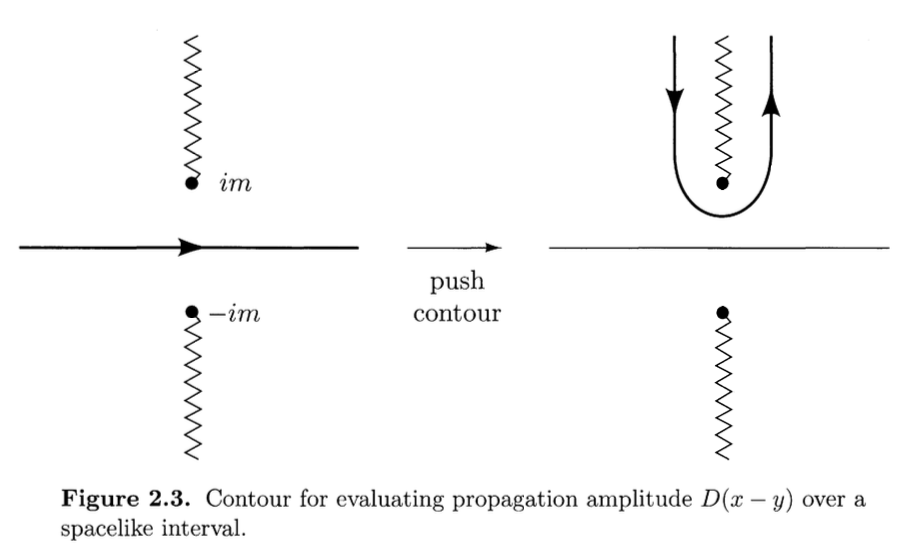
\includegraphics[width=1\textwidth]{PeskinQFT_Sec2-4_fig/fig2-3.png}
\end{figure}

\begin{itemize}
  \item 光円錐の外側でも場の振幅は指数的に減衰するがゼロではない.
  \item 因果性を議論する際の本質的な問いは, 「粒子が空間的間隔を越えて伝播できるか」ではなく, 「一方の測定が他方に影響を与えるかどうか」である.
  \item 具体的には, 場 $\phi(x)$ の測定が $\phi(y)$ に影響を与えるかを調べる必要がある.
  \item そのためには, 交換子 $[\phi(x), \phi(y)]$ を計算し, その値がゼロかどうかを見る.
  \item 交換子がゼロであれば, 互いの測定は影響を与え合わず, 因果性が保たれる.
  \item 特に, $(x - y)^2 < 0$ (Spacelike) で交換子がゼロであることが因果性の保証となる.
  \item $\phi(x)$ の時間微分 $\pi(x) = \partial \phi / \partial t$ のような任意の関数との可換子もゼロであるべき.
  \item 式(2.20) より, $x^0 = y^0$ (同時刻) ではすでに交換子がゼロであることは確認済み.
  \begin{equation*}
    [\phi(\mathbf{x}), \phi(\mathbf{y})] = [\pi(\mathbf{x}), \pi(\mathbf{y})] = 0 \tag{2.20}
  \end{equation*}
  \item ここでは, それをより一般の場合 (任意の $x$, $y$) に拡張して計算を行う.
\end{itemize}
\begin{align*}
[\phi(x), \phi(y)] &= \int \frac{d^3 p}{(2\pi)^3} \frac{1}{\sqrt{2E_{\mathbf{p}}}} \int \frac{d^3 q}{(2\pi)^3} \frac{1}{\sqrt{2E_{\mathbf{q}}}} \\
&\quad \times \left[ \left( a_{\mathbf{p}} e^{-ip \cdot x} + a_{\mathbf{p}}^\dagger e^{ip \cdot x} \right), \left( a_{\mathbf{q}} e^{-iq \cdot y} + a_{\mathbf{q}}^\dagger e^{iq \cdot y} \right) \right] \\
&= \int \frac{d^3 p}{(2\pi)^3} \frac{1}{2E_{\mathbf{p}}} \left( e^{-ip \cdot (x - y)} - e^{ip \cdot (x - y)} \right) \\
&= D(x - y) - D(y - x) \label{2.53}\tag{2.53}
\end{align*}

\color{blue}
生成消滅演算子の交換子の計算:
\begin{align*}
  [a_{\mathbf{p}}, a_{\mathbf{q}}^\dagger] &= (2\pi)^3 \delta^{(3)}(\mathbf{p} - \mathbf{q}) \tag{2-4.g1}\\
  [a_{\mathbf{p}}, a_{\mathbf{q}}] &= [a_{\mathbf{p}}^\dagger, a_{\mathbf{q}}^\dagger] = 0 \tag{2-4.g2}
\end{align*}
から \eqref{2.53} での計算を簡単に確認する. まず, 
\begin{align*}
  &\left[ \left( a_{\mathbf{p}} e^{-ip \cdot x} + a_{\mathbf{p}}^\dagger e^{ip \cdot x} \right), \left( a_{\mathbf{q}} e^{-iq \cdot y} + a_{\mathbf{q}}^\dagger e^{iq \cdot y} \right) \right] \\
  &\quad \hspace{3cm} = [a_{\mathbf{p}}, a_{\mathbf{q}}] e^{-ip \cdot x} e^{-iq \cdot y} + [a_{\mathbf{p}}, a_{\mathbf{q}}^\dagger] e^{-ip \cdot x} e^{iq \cdot y} \\
  &\quad \hspace{4cm} + [a_{\mathbf{p}}^\dagger, a_{\mathbf{q}}] e^{ip \cdot x} e^{-iq \cdot y} + [a_{\mathbf{p}}^\dagger, a_{\mathbf{q}}^\dagger] e^{ip \cdot x} e^{iq \cdot y} \tag{2-4.g3}\\
  &\quad \hspace{3cm} = (2\pi)^3 \delta^{(3)}(\mathbf{p} - \mathbf{q}) e^{-ip \cdot x} e^{iq \cdot y} - (2\pi)^3 \delta^{(3)}(\mathbf{p} - \mathbf{q}) e^{ip \cdot x} e^{-iq \cdot y} \tag{2-4.g4}\\
\end{align*}
となるので, デルタ関数を実行すれば,
\begin{align*}
  [\phi(x), \phi(y)] &= \int \frac{d^3 p}{(2\pi)^3} \frac{1}{2E_{\mathbf{p}}} \left( e^{-ip \cdot (x - y)} - e^{ip \cdot (x - y)} \right). \tag{2-4.g5}
\end{align*}
$D(x-y)$ の定義は, \eqref{2.50} より,
\begin{equation*}
  D(x - y) = \langle 0 | \phi(x) \phi(y) | 0 \rangle = \int \frac{d^3 p}{(2\pi)^3} \frac{1}{2E_p} e^{-ip \cdot (x - y)} \tag{2.50}
  \end{equation*}
なので, \eqref{2.53} が直ちに得られる.
\vskip\baselineskip
\color{black}

Klein-Gordon 理論においては, \textbf{因果性 (causality)}が重要な物理的要請である. 特に, 場の交換子が空間的に離れた点でゼロになることは, 測定の非干渉性, すなわち因果性の保存を意味する.

\subsection*{時空間隔による場合分け}
まず, 時空間隔 $(x - y)^2$ の符号によって, 次のように状況が異なる:
\begin{itemize}
  \item $(x - y)^2 < 0$ (Spacelike):
  \begin{itemize}
    \item Lorentz 変換によって $(x - y) \to -(x - y)$ を行うことが可能.
    \item 各項は Lorentz 不変であるため, 二項が打ち消し合い, 交換子はゼロ.
    \item よって, 光円錐の外では因果性が保持される (Figure 2.4 参照).
  \end{itemize}

  \begin{figure}[H]
    \centering
    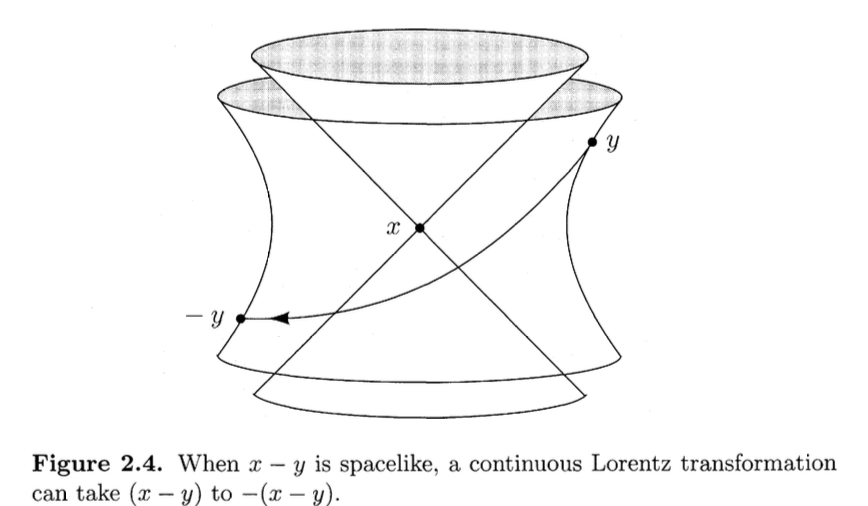
\includegraphics[width=1\textwidth]{PeskinQFT_Sec2-4_fig/fig2-4.png}
\end{figure}

  \item $(x - y)^2 > 0$ (Timelike):
  \begin{itemize}
    \item 上記のような変換を行う連続的な Lorentz 変換は存在しない.\\
    \textcolor{blue}{※時間反転を用いないといけないので, timelike の場合はこのような変換はできない. 詳細は九後「ゲージ場の量子論I」の1章を参照.}
    \item 交換子はゼロではないが, $e^{-imt} - e^{imt}$ のように急速に減衰.\\
    \textcolor{blue}{※$e^{-imt} - e^{imt} = 2i\sin(mt)$ より, $t \to \infty$ でもゼロにならない.}
  \end{itemize}

  \item 特別な場合 $x = y$:
  \begin{itemize}
    \item 交換子は厳密にゼロである.
  \end{itemize}
\end{itemize}
したがって, Klein-Gordon 理論では光円錐の外での因果性は守られている. これをより厳密に理解するには, \textbf{複素 Klein-Gordon 場}の導入が必要である.
\subsection*{複素スカラー場と電荷}
複素 Klein-Gordon 場の導入によって, 粒子と反粒子の励起が区別可能となる. 特に, 電荷保存則を導入するには, $\phi(x)$ を実数ではなく複素数値の場として扱う必要がある.\\
このとき:
\begin{itemize}
  \item $\phi(x)$ は正電荷の粒子を生成し, 負電荷の粒子を消滅させる.
  \item $\phi^\dagger(x)$ は負電荷の粒子を生成し, 正電荷の粒子を消滅させる.
\end{itemize}
交換子 $[\phi(x), \phi^\dagger(y)]$ は光円錐の外でゼロではないが, 物理的には\textbf{干渉を打ち消す必要がある}.
\subsection*{2つの伝播過程と因果性の確保}
式 \eqref{2.53} に現れる 2 項は, 次の 2 つの過程を表している:
\begin{itemize}
  \item 第1項:負電荷を持つ粒子が $y$ から $x$ に伝播する.
  \item 第2項:正電荷を持つ粒子が $x$ から $y$ に伝播する.
\end{itemize}
この2過程が打ち消し合うためには, 両方の粒子が存在し, 同じ質量を持っていなければならない. 量子場理論では, \textbf{すべての粒子には同じ質量で逆の量子数(この場合は電荷)を持つ対応する反粒子が存在する}. 実数値の Klein-Gordon 場では, 粒子は自分自身が反粒子である.
\subsection*{Klein-Gordon 伝播子}
交換子 $[\phi(x), \phi(y)]$ をさらに調べてみる. これは $c$-number (定数) なので,
\begin{equation*}
[\phi(x), \phi(y)] = \langle 0 | [\phi(x), \phi(y)] | 0 \rangle
\end{equation*}
と書け,次のような4次元積分として表すことができる (ただし, $x^0 > y^0$ を仮定):
\begin{align*}
\langle 0 | [\phi(x), \phi(y)] | 0 \rangle &= \int \frac{d^3 p}{(2\pi)^3} \frac{1}{2E_p} \left( e^{-ip \cdot (x - y)} - e^{ip \cdot (x - y)} \right) \\
&= \int \frac{d^3 p}{(2\pi)^3} \left\{ \left.\frac{1}{2E_p} e^{-ip \cdot (x - y)}\right|_{p^0 = E_{\mathbf{p}}} - \left.\frac{1}{2E_p} e^{-ip \cdot (x - y)}\right|_{p^0 = -E_{\mathbf{p}}} \right\}\\
&= \int \frac{d^3 p}{(2\pi)^3} \int \frac{dp^0}{2\pi i}\frac{-1}{p^2 -m^2} e^{-ip \cdot (x - y)},\hspace{0.5cm} (x^0 > y^0) \label{2.54}\tag{2.54}
\end{align*}
\textcolor{blue}{2行目の式は指数関数の中の $p^0$ を明示的に書いている.\\
ここで $p \cdot (x - y) = p^0 (x^0 - y^0) - \mathbf{p} \cdot (\mathbf{x} - \mathbf{y})$ と書き換えることで, 後に複素積分の極として $p^0 = \pm E_{\mathbf{p}}$ が現れることを意識している. そして\eqref{2.54} の2行目から3行目の変形は場の交換関係やグリーン関数の構造を理解していないと思いつきにくい変形なので, 今回は3行目から2行目の式になることを留数定理を用いて確認しておく.}\\


最後のステップでは, $p^0$ に関する積分を以下の積分経路に沿って行う:

\begin{figure}[H]
    \centering
    \begin{tikzpicture}
      \draw[gray!50](1,0)--(11,0);
      \draw[line width=1pt,-{Stealth[length=3mm]}](1,0)--(2,0);
      \fill(3.5,0)node[below]{$-E_{\textbf{p}}$}circle[radius=0.05];
      \fill(8.7,0)node[below]{$+E_{\textbf{p}}$}circle[radius=0.05];
      \draw[line width=1pt](1,0)--(2.8,0)arc(180:0:.7)--++(3.8,0)arc(180:0:.7)--++(1.8,0);
      \draw[line width=1pt,-{Stealth[length=3mm]}](9.4,0)--(10.5,0);
      \draw[thick,gray!80](6.1,1.5)--(6.1,-1.5);
    \end{tikzpicture}
\end{figure}

\color{blue}
と図があるが, 実軸上に極があると計算が面倒なので, 極を $i\epsilon$ だけ実軸から下げて時計周りに積分経路を閉じる. よって実際の経路はこのように取ると良い.

\begin{figure}[H]
  \centering
  \begin{tikzpicture}
    \color{blue}
    %change color as you like
    \def\c{blue}
    \draw[thick,-{Stealth[length=2mm]},\c](0.5,0)--(5.5,0);
    \draw[thick,-{Stealth[length=2mm]},\c](3,-2.5)--(3,1);
    \draw[very thick,-{Stealth[length=4mm]},\c](1,0)--(2.5,0);
    \draw[very thick,-{Stealth[length=4mm]},\c](2.2,0)--(4,0);
    \draw[very thick,-{Stealth[length=4mm]},\c](3.8,0)--(5,0)arc(0:-80:2cm);
    \draw[very thick](1,0)arc(180:285:2cm);
    \fill(2,-.5)node[below]{\scalebox{.8}{$-\textrm{E}_{\mathbf{p}}-i\varepsilon$}}circle[radius=0.08];
    \fill(4,-.5)node[below]{\scalebox{.8}{$\textrm{E}_{\mathbf{p}}-i\varepsilon$}}circle[radius=0.08];
  \end{tikzpicture}
\end{figure}


実際にこの経路で \eqref{2.54} の3行目から2行目の式を確認する. $(x^0 > y^0)$ のとき,
\begin{align*}
  \int \frac{d^3 p}{(2\pi)^3} \int \frac{dp^0}{2\pi i}\frac{-1}{p^2 -m^2} e^{-ip \cdot (x - y)} &= \int \frac{d^3 p}{(2\pi)^3} \int \frac{dp^0}{2\pi i}\frac{-1}{p^2 -m^2} e^{-ip \cdot (x - y)} \tag{2-4.h1}\\
  = \int \frac{d^3 p}{(2\pi)^3} \int \frac{dp^0}{2\pi i}&\frac{-1}{(p^0)^2 - \mathbf{p}^2 -m^2} e^{-i(p^0(x^0 - y^0) - \mathbf{p} \cdot (\mathbf{x} - \mathbf{y}))} \tag{2-4.h2}\\
  = \int \frac{d^3 p}{(2\pi)^3} e^{i\mathbf{p}\cdot(\mathbf{x} - \mathbf{y})} \int& \frac{dp^0}{2\pi i}\frac{-1}{(p^0)^2 - E_{\mathbf{p}}^2} e^{-ip^0(x^0 - y^0)}\quad(E_{\mathbf{p}} = \sqrt{\mathbf{p}^2 + m^2}) \tag{2-4.h3}\\
  = \int \frac{d^3 p}{(2\pi)^3} e^{i\mathbf{p}\cdot(\mathbf{x} - \mathbf{y})} \int &\frac{dp^0}{2\pi i}\frac{-1}{(p^0 - E_{\mathbf{p}}) (p^0 + E_{\mathbf{p}})} e^{-ip^0(x^0 - y^0)} \label{2-4.h4}\tag{2-4.h4}\\
  = \int \frac{d^3 p}{(2\pi)^3} e^{i\mathbf{p}\cdot(\mathbf{x} - \mathbf{y})} \lim_{\epsilon \to 0}&\int \frac{dp^0}{2\pi i}\frac{-e^{-ip^0(x^0 - y^0)}}{(p^0 - (E_{\mathbf{p}} - i\epsilon)) (p^0 - (-E_{\mathbf{p}} - i\epsilon))} \label{2-4.h5}\tag{2-4.h5}\\
  = \int \frac{d^3 p}{(2\pi)^3} e^{i\mathbf{p}\cdot(\mathbf{x} - \mathbf{y})} \lim_{\epsilon \to 0}&\left( -\frac{-e^{-i(E_{\mathbf{p}} - i\epsilon)(x^0 - y^0)}}{(E_{\mathbf{p}} - i\epsilon)-(-E_{\mathbf{p}} - i\epsilon)} - \frac{-e^{-i(-E_{\mathbf{p}} - i\epsilon)(x^0 - y^0)}}{(-E_{\mathbf{p}} - i\epsilon)-(E_{\mathbf{p}} - i\epsilon)} \right) \tag{2-4.h6}\\
  = \int \frac{d^3 p}{(2\pi)^3} e^{i\mathbf{p}\cdot(\mathbf{x} - \mathbf{y})} \lim_{\epsilon \to 0}&\left( \frac{e^{-i(E_{\mathbf{p}} - i\epsilon)(x^0 - y^0)}}{2E_{\mathbf{p}}} - \frac{e^{-i(-E_{\mathbf{p}} - i\epsilon)(x^0 - y^0)}}{2E_{\mathbf{p}}} \right) \tag{2-4.h7}\\
  = \int \frac{d^3 p}{(2\pi)^3} e^{i\mathbf{p}\cdot(\mathbf{x} - \mathbf{y})} &\left( \frac{e^{-iE_{\mathbf{p}}(x^0 - y^0)}}{2E_{\mathbf{p}}} - \frac{e^{-i(-E_{\mathbf{p}})(x^0 - y^0)}}{2E_{\mathbf{p}}} \right) \tag{2-4.h8}\\
  = \int \frac{d^3 p}{(2\pi)^3} &\left\{ \left.\frac{1}{2E_p} e^{-ip \cdot (x - y)}\right|_{p^0 = E_{\mathbf{p}}} - \left.\frac{1}{2E_p} e^{-ip \cdot (x - y)}\right|_{p^0 = -E_{\mathbf{p}}} \right\} \tag{2-4.h9}
\end{align*}
\eqref{2-4.h4} から \eqref{2-4.h5} の変形は, 留数定理を用いている:
\begin{equation*}
  \int \frac{f(z)}{2\pi i} dp^0 = \sum \text{Res}(f(z), a_i)
\end{equation*}
ここで $a_i$ は $f(z)$ の極を表す. 


\color{black}

$x^0 > y^0$ の場合, 下側の輪郭で積分経路を閉じて2つのポールを拾い, \eqref{2.54} の最後の結果が得られる. 一方, $x^0 < y^0$ の場合は上側で閉じてゼロとなる. よって, ポールの処理を含めた式は以下の量として定義される:

\begin{equation*}
D_R(x - y) \equiv \theta(x^0 - y^0)\, \langle 0 | [\phi(x), \phi(y)] | 0 \rangle \tag{2.55}
\end{equation*}

この量をより深く理解するために, 以下の計算を行う:

\begin{align*}
(\partial^2 + m^2) D_R(x - y) &= \left( \partial^2 \theta(x^0 - y^0) \right) \langle 0 | [\phi(x), \phi(y)] | 0 \rangle \notag \\
&\quad + 2 \left( \partial_\mu \theta(x^0 - y^0) \right) \left( \partial^\mu \langle 0 | [\phi(x), \phi(y)] | 0 \rangle \right) \notag \\
&\quad + \theta(x^0 - y^0) \left( \partial^2 + m^2 \right) \langle 0 | [\phi(x), \phi(y)] | 0 \rangle \notag \\
&= -\delta(x^0 - y^0) \langle 0 | [\pi(x), \phi(y)] | 0 \rangle \notag \\
&\quad + 2\delta(x^0 - y^0) \langle 0 | [\pi(x), \phi(y)] | 0 \rangle + 0 \notag \\
&= -i\delta^{(4)}(x - y) \label{2.56}\tag{2.56}
\end{align*}

\color{blue}
\begin{proof}
\eqref{2.56} の計算確認:\\
Leibniz則から
\begin{equation*}
  \partial^2 (fg) = (\partial^2 f)g + 2\partial f \partial g + f(\partial^2 g) \tag{2-4.i1}
\end{equation*}
が成り立つので
\begin{align*}
  (\partial^2 + m^2) D_R(x - y) &= (\partial^2 + m^2) \theta(x^0 - y^0)\, \langle 0 | [\phi(x), \phi(y)] | 0 \rangle \tag{2-4.i2}\\
  &= (\partial^2 \theta(x^0 - y^0))\, \langle 0 | [\phi(x), \phi(y)] | 0 \rangle \\
  &\quad + 2(\partial_\mu \theta(x^0 - y^0))\, \langle 0 | [\partial^\mu \phi(x), \phi(y)] | 0 \rangle\\
  &\quad + \theta(x^0 - y^0)\,\partial^2\, \langle 0 | [\phi(x), \phi(y)] | 0 \rangle\\
  &\quad + \theta(x^0 - y^0)\, m^2\, \langle 0 | [\phi(x), \phi(y)] | 0 \rangle \tag{2-4.i3}\\
  &= \left( \partial^2 \theta(x^0 - y^0) \right) \langle 0 | [\phi(x), \phi(y)] | 0 \rangle \notag \\
  &\quad + 2 \left( \partial_\mu \theta(x^0 - y^0) \right) \left( \partial^\mu \langle 0 | [\phi(x), \phi(y)] | 0 \rangle \right) \notag \\
  &\quad + \theta(x^0 - y^0) \left( \partial^2 + m^2 \right) \langle 0 | [\phi(x), \phi(y)] | 0 \rangle \tag{2-4.i4}
\end{align*}
ここで各項について計算を行う:
\begin{align*}
  \left( \partial^2 \theta(x^0 - y^0) \right) \langle 0 | [\phi(x), \phi(y)] | 0 \rangle &= \left( (\partial_0^2 - \nabla^2) \theta(x^0 - y^0) \right) \langle 0 | [\phi(x), \phi(y)] | 0 \rangle \tag{2-4.i5}\\
  = \left( \partial_0 \partial^0 \theta(x^0 - y^0) \right)& \langle 0 | [\phi(x), \phi(y)] | 0 \rangle\quad(\because \nabla \theta(x^0 - y^0) = 0) \tag{2-4.i6}\\
  = \left( \partial_0 (g^{00} \partial_0) \delta(x^0 - y^0) \right) &\langle 0 | [\phi(x), \phi(y)] | 0 \rangle \quad(\text{添え字の上げ下げ}) \tag{2-4.i7}\\
  = \left( \partial_0 \delta(x^0 - y^0) \right) &\langle 0 | [\phi(x), \phi(y)] | 0 \rangle \quad\left(\because \delta (x) = \frac{d}{dx} \theta(x)\right) \tag{2-4.i8}
\end{align*}
\begin{align*}
  2(\partial_\mu \theta(x^0 - y^0))\, \partial^\mu \langle 0 | [\phi(x), \phi(y)] | 0 \rangle &= 2(\partial_\mu \theta(x^0 - y^0))\, \langle 0 | [\partial^\mu \phi(x), \phi(y)] | 0 \rangle \tag{2-4.i8}\\
  &= 2(\partial_0 \theta(x^0 - y^0))\, \partial^0 \langle 0 | [\phi(x), \phi(y)] | 0 \rangle\\
  &\quad + 2(\underline{\partial_i \theta(x^0 - y^0)})\, \partial^i \langle 0 | [\phi(x), \phi(y)] | 0 \rangle \tag{2-4.i9}\\
  &\quad \hspace{1.5cm} \text{= 0}\\
  &= 2(\partial_0 \theta(x^0 - y^0))\, \partial^0 \langle 0 | [\phi(x), \phi(y)] | 0 \rangle \tag{2-4.i10}\\
  &= 2\delta(x^0 - y^0)\, \langle 0 | [\partial^0 \phi(x), \phi(y)] | 0 \rangle \tag{2-4.i11}\\
  &= 2\delta(x^0 - y^0)\, \langle 0 | [g^{00}\underline{\partial_0 \phi(x)}, \phi(y)] | 0 \rangle \tag{2-4.i12}\\
  &\quad \hspace{2.5cm} \partial_0 \phi(x) = \pi(x)\\
  &= 2\delta(x^0 - y^0)\, \langle 0 | [ \pi(x), \phi(y)] | 0 \rangle \tag{2-4.i13}\\
\end{align*}
\begin{align*}
  \theta(x^0 - y^0) \left( \partial^2 + m^2 \right) \langle 0 | [\phi(x), \phi(y)] | 0 \rangle &= \theta(x^0 - y^0) \left( \partial^2 + m^2 \right) [\phi(x), \phi(y)] \langle 0 | 0 \rangle \tag{2-4.i14}\\
  &= \theta(x^0 - y^0) \left( \partial^2 + m^2 \right) [\phi(x), \phi(y)] \tag{2-4.i15}\\
  &= \theta(x^0 - y^0) \left( \partial^2 + m^2 \right) (\phi(x) \phi(y) - \phi(y) \phi(x)) \tag{2-4.i16}
\end{align*}
相互作用のない自由場を考えているので, Klein-Gordon 方程式 $(\partial^2 + m^2) \phi = 0$ となり, これを用いると
\begin{equation*}
  \theta(x^0 - y^0) \left( \partial^2 + m^2 \right) \langle 0 | [\phi(x), \phi(y)] | 0 \rangle = 0 \tag{2-4.i17}
\end{equation*}
したがって,
\begin{align*}
  (\partial^2 + m^2) D_R(x - y) &= \underline{\left( \partial_0 \delta(x^0 - y^0) \right) \langle 0 | [\phi(x), \phi(y)] | 0 \rangle} \notag \\
  &\quad + 2 \delta(x^0 - y^0) \langle 0 | [\pi(x), \phi(y)] | 0 \rangle \tag{2-4.i18}\\
  &= \delta(x^0 - y^0) \langle 0 | [\phi(x), \phi(y)] | 0 \rangle - \delta(x^0 - y^0) \partial_0\langle 0 | [\phi(x), \phi(y)] | 0 \rangle\\
  &\quad \hspace{1cm} + 2 \delta(x^0 - y^0) \langle 0 | [\pi(x), \phi(y)] | 0 \rangle \tag{2-4.i20}\\
  &= - \delta(x^0 - y^0) \partial_0\langle 0 | [\phi(x), \phi(y)] | 0 \rangle\\
  &\quad + 2 \delta(x^0 - y^0) \langle 0 | [\pi(x), \phi(y)] | 0 \rangle \quad(\because [\phi(x), \phi(y)] = 0)\tag{2-4.i21}\\
  &= - \delta(x^0 - y^0) \langle 0 | [\pi(x), \phi(y)] | 0 \rangle \\
  &\quad + 2 \delta(x^0 - y^0) \langle 0 | [\pi(x), \phi(y)] | 0 \rangle \quad(\because \partial_0 \phi(x) = \pi(x)) \tag{2-4.i22}\\
  &= \delta(x^0 - y^0) \langle 0 | [\pi(x), \phi(y)] | 0 \rangle \tag{2-4.i23}\\
  &= -\delta(x^0 - y^0) i\delta^{(3)}(\mathbf{x} - \mathbf{y}) \langle 0 | 0 \rangle \quad(\because [\pi(x), \phi(y)] = -i\delta^{(3)}(\mathbf{x} - \mathbf{y})) \tag{2-4.i24}\\
  &= -i\delta^{(4)}(x - y) \quad(\because \langle 0 | 0 \rangle = 1) \tag{2-4.i25}
\end{align*}
\end{proof}
\color{black}

これは $D_R(x - y)$ が Klein-Gordon 演算子のグリーン関数である.\par
\color{blue} 
グリーン関数とは?\\
次のような線形方程式を考える:
\begin{equation*}
  Lu(x) = f(x) \tag{2-4.j1}
\end{equation*}
ここで,
\begin{itemize}
  \item $L$:線形微分演算子
  \item $f(x)$:ソース項 (相互作用など外部の力)
  \item $u(x)$:求めたい関数 (応答)
\end{itemize}
このとき, グリーン関数 $G(x, y)$ は次のように定義される:
\begin{equation*}
  LG(x, y) = \delta(x - y) \tag{2-4.j2}
\end{equation*}
グリーン関数を使えば, 元の方程式の解 $u(x)$ は次のように求められる:
\begin{equation*}
  u(x) = \int d^4 y \, G(x, y) f(y) \tag{2-4.j3}
\end{equation*}
つまり, ソースをグリーン関数で重ね合わせることで解が得られる. \eqref{2.56} では係数に $-i$ があるが, これは $[\pi(x), \phi(y)] = -i\delta^{(4)}(x - y)$ という場の量子論における交換関係の性質に由来するものである.
\vskip\baselineskip
\color{black}
特に, $x^0 < y^0$ で消えるので, \textbf{遅延グリーン関数} (retarded Green's function) である.
式 \eqref{2.54} を導出していなかったとしても, フーリエ変換により次のように得られる:
\begin{equation*}
D_R(x - y) = \int \frac{d^4 p}{(2\pi)^4} e^{-ip \cdot (x - y)} \, \widetilde{D}_R(p) \label{2.57}\tag{2.57}
\end{equation*}
ここで, $\widetilde{D}_R(p)$ は以下を満たす:
\begin{equation*}
(-p^2 + m^2)\, \widetilde{D}_R(p) = -i
\end{equation*}
したがって, 即座に次の結果が得られる:
\begin{equation*}
D_R(x - y) = \int \frac{d^4 p}{(2\pi)^4} \frac{i}{p^2 - m^2} e^{-ip \cdot (x - y)} \label{2.58}\tag{2.58}
\end{equation*}
\color{blue}
\eqref{2.56} より, デルタ関数をフーリエ変換すると,
\begin{equation*}
  (\partial^2 + m^2) D_R(x - y) = -i\delta(x - y) = \int \frac{d^4 p}{(2\pi)^4}\, e^{-ip \cdot (x - y)} \label{2-4.k1}\tag{2-4.k1}
\end{equation*}
また, \eqref{2.57} より,
\begin{align*}
  (\partial^2 + m^2) D_R(x - y) &= (\partial^2 + m^2) \int \frac{d^4 p}{(2\pi)^4} e^{-ip \cdot (x - y)} \, \widetilde{D}_R(p) \tag{2-4.k2}\\
  &= \int \frac{d^4 p}{(2\pi)^4} \left( -p^2 + m^2 \right) e^{-ip \cdot (x - y)} \, \widetilde{D}_R(p) \label{2-4.k3}\tag{2-4.k3}
\end{align*}
よって, \eqref{2-4.k1} と \eqref{2-4.k3} より,
\begin{equation*}
  \int \frac{d^4 p}{(2\pi)^4} \left( -p^2 + m^2 \right) e^{-ip \cdot (x - y)} \, \widetilde{D}_R(p) = \int \frac{d^4 p}{(2\pi)^4}\, e^{-ip \cdot (x - y)} \tag{2-4.k4}
\end{equation*}
これより,
\begin{equation*}
  \widetilde{D}_R(p) = \frac{i}{p^2 - m^2} \tag{2-4.k5}
\end{equation*}
これは $e^{-ip \cdot (x - y)}$ がフーリエ変換における基底となっているので, 係数が等しいと言える. 一般に $\displaystyle \int f(x)dx = \int g(x)dx \Longrightarrow f(x) \neq g(x)$ であることに注意.
\vskip\baselineskip
\color{black}


式 \eqref{2.58} の $p^0$ 積分は, 4通りの異なる積分経路に従って評価することができる. そのうち \eqref{2.54} で用いられたのは1つにすぎない. 第4章では, 異なる極の取り扱い (pole prescription) を見つけるが, その1つが以下のようなものである:

\begin{figure}[H]
    \centering
    \begin{tikzpicture}
      \draw[gray!50](1,0)--(11,0);
      \draw[line width=1pt,-{Stealth[length=3mm]}](1,0)--(2,0);
      \fill(3.5,0)node[above]{$-E_{\textbf{p}}$}circle[radius=0.05];
      \fill(8.7,0)node[below]{$+E_{\textbf{p}}$}circle[radius=0.05];
      \draw[line width=1pt](1,0)--(2.8,0)arc(180:360:.7)--++(3.8,0)arc(180:0:.7)--++(1.8,0);
      \draw[line width=1pt,-{Stealth[length=3mm]}](9.4,0)--(10.5,0);
      \draw[thick,gray!80](6.1,1.5)--(6.1,-1.5);
    \end{tikzpicture}
\end{figure}  

これは非常に有用であり, \textbf{ファsインマン処方 (Feynman prescription)}と呼ばれる. 覚えやすい表記としては次のように書ける:
\begin{equation*}
D_F(x - y) \equiv \int \frac{d^4p}{(2\pi)^4} \frac{i}{p^2 - m^2 + i\epsilon} e^{-ip \cdot (x - y)} \label{2.59}\tag{2.59}
\end{equation*}
このとき, 極は $p^0 = \pm(E_p - i\epsilon)$ にあり, 適切に実軸の上下にずれている. $x^0 > y^0$ のときは, 下側の経路で閉じることで $D(x - y)$ (\eqref{2.50}) と一致する. $x^0 < y^0$ のときは, 上側で閉じて $x$ と $y$ を入れ替えた形の結果が得られる.

したがって,

\begin{equation*}
D_F(x - y) =
\begin{cases}
D(x - y), & \text{if } x^0 > y^0 \\
D(y - x), & \text{if } x^0 < y^0
\end{cases}
\end{equation*}
これは次のようにも表現できる:
\begin{align*}
D_F(x - y)
&= \theta(x^0 - y^0)\, \langle 0 | \phi(x) \phi(y) | 0 \rangle + \theta(y^0 - x^0)\, \langle 0 | \phi(y) \phi(x) | 0 \rangle \notag \\
&\equiv \langle 0 | T\phi(x) \phi(y) | 0 \rangle \label{2.60}\tag{2.60}
\end{align*}
最後の式においては, \textbf{時間順序演算子} $T$ を定義しており, これは演算子を時間的に遅いものを右側に並べるように順序付けすることを意味する.\\
$(\Box + m^2)$ を \eqref{2.60} に作用させることで, $D_F$ が Klein-Gordon 演算子のグリーン関数であることを直接確認することができる.

\bigskip

\eqref{2.59} および \eqref{2.60} は, 本章における最も実用的で重要な結果である.\\
グリーン関数 $D_F(x - y)$ は, Klein-Gordon 粒子に対する \textbf{ファインマンプロパゲータ(Feynman propagator)} と呼ばれる. ファインマンプロパゲータはファインマン則における基本要素で, 内部線に対応する数式として $D_F(x - y)$ やそのフーリエ変換 $\widetilde{D}_F(p)$ が用いられ, 仮想粒子の伝播を表す. とはいえ, 我々はまだ実際の物理的計算を行うには程遠い段階にある. ここまでは自由 Klein-Gordon 理論についてのみ議論しており, 場の方程式は線形で, 相互作用は存在しない. このような理論では, 個々の粒子は孤立しており, 他の粒子の存在に無関心である. 他の粒子が存在する可能性や, 散乱・崩壊といった物理的過程を議論する余地がない.

\subsection*{古典的ソースによる粒子生成}
ここで扱うことができる相互作用の一種として, Klein-Gordon 場が外部の古典的場 $j(x)$ に結合している場合がある. すなわち, 以下の場の方程式を考える:
\begin{equation*}
(\Box + m^2) \phi(x) = j(x) \label{2.61}\tag{2.61}
\end{equation*}
ここで $j(x)$ は空間と時間の既知の関数であり, 有限時間のみ非ゼロであるとする. 真空状態から始めて, $j(x)$ がオン・オフされた後に何が起こるかを調べる.\\
場の方程式 \eqref{2.61} は次のラグランジアンから導出される:
\begin{equation*}
\mathcal{L} = \frac{1}{2} (\partial_\mu \phi)^2 - \frac{1}{2} m^2 \phi^2 + j(x) \phi(x) \tag{2.62}
\end{equation*}
$j(x)$ が有限時間のみ作用する場合, 場の方程式を直接解くのが簡単である. $j(x)$ がオンになる前, $\phi(x)$ は以下の形式を取る:
\begin{equation*}
\phi_0(x) = \int \frac{d^3 p}{(2\pi)^3} \frac{1}{\sqrt{2E_p}} \left( a_{\mathbf{p}} e^{-ip \cdot x} + a_{\mathbf{p}}^\dagger e^{ip \cdot x} \right)
\end{equation*}
ソースが存在しなければ, これは常に正しい解となる. ソースが存在する場合, 運動方程式の解は遅延グリーン関数 $D_R$ を用いて以下のように構成できる:
\begin{align*}
\phi(x) &= \phi_0(x) + i \int d^4 y\, D_R(x - y) j(y) \notag \\
&= \phi_0(x) + i \int d^4 y \int \frac{d^3 p}{(2\pi)^3} \frac{1}{2E_p} \theta(x^0 - y^0) \left( e^{-ip \cdot (x - y)} - e^{ip \cdot (x - y)} \right) j(y) \label{2.63}\tag{2.63}
\end{align*}
すべての $j$ が過去に存在する場合, $\theta$ 関数は積分領域全体で1となる. このとき, $\phi(x)$ は $j$ のフーリエ変換のみを含む:
\begin{equation*}
\tilde{j}(p) = \int d^4 y\, e^{ip \cdot y} j(y)
\end{equation*}
ここで, 4運動量 $p$ は $p^2 = m^2$ を満たすように評価される. 正周波数の項 ($a_{\mathbf{p}}$) と負周波数の項 ($a_{\mathbf{p}}^\dagger$) を自然にまとめると, 以下の式が得られる:
\begin{equation*}
\phi(x) = \int \frac{d^3 p}{(2\pi)^3} \frac{1}{\sqrt{2E_p}} \left\{ \left( a_{\mathbf{p}} + \frac{i}{\sqrt{2E_p}} \tilde{j}(p) \right) e^{-ip \cdot x} + \text{h.c.} \right\} \label{2.64}\tag{2.64}
\end{equation*}

\color{blue}
\begin{proof}
\eqref{2.64} の導出.\\
すべての $j$ が過去に存在する場合, $\theta (x^0 - y^0)$ は積分領域全体で1となるので, \eqref{2.63} より,
\begin{align*}
  \phi(x) &= \phi_0(x) + i \int d^4 y \int \frac{d^3 p}{(2\pi)^3} \frac{1}{2E_p} \left( e^{-ip \cdot (x - y)} - e^{ip \cdot (x - y)} \right) j(y) \tag{2-4.l1}\\
  &= \phi_0(x) + i \int \frac{d^3 p}{(2\pi)^3} \frac{1}{2E_p} \left( e^{-ip \cdot x} \int d^4 y\, e^{ip \cdot y} j(y) - e^{ip \cdot x} \int d^4 y\, e^{-ip \cdot y} j(y) \right) \tag{2-4.l2}\\
  &= \phi_0(x) + i \int \frac{d^3 p}{(2\pi)^3} \frac{1}{2E_p} \left( e^{-ip \cdot x} \tilde{j}(p) - e^{ip \cdot x} \tilde{j}^{*}(p) \right) \quad(\because j(-p) = j^{*}(p)) \tag{2-4.l3}\\
  &= \int \frac{d^3 p}{(2\pi)^3} \frac{1}{\sqrt{2E_p}} \left( a_{\mathbf{p}} e^{-ip \cdot x} + a_{\mathbf{p}}^\dagger e^{ip \cdot x} \right)\\
  &\quad + i \int \frac{d^3 p}{(2\pi)^3} \frac{1}{2E_p} \left( e^{-ip \cdot x} \tilde{j}(p) - e^{ip \cdot x} \tilde{j}^{*}(p) \right) \tag{2-4.l4}\\
  &= \int \frac{d^3 p}{(2\pi)^3} \frac{1}{\sqrt{2E_p}} \left\{ \left( a_{\mathbf{p}} + \frac{i}{\sqrt{2E_p}} \tilde{j}(p) \right) e^{-ip \cdot x} + \text{h.c.} \right\} \tag{2-4.l5}
\end{align*}
ここで, h.c. は Hermite 共役を表す.
\end{proof}
\color{black}

ここから, $j(x)$ が作用したあとのハミルトニアンの形を推測することができる.\\
すなわち, $a_{\mathbf{p}}$ を
\begin{equation*}
a_{\mathbf{p}} \rightarrow a_{\mathbf{p}} + \frac{i}{\sqrt{2E_p}} \tilde{j}(p)
\end{equation*}
と置き換えることで, ハミルトニアンは次のようになる:
\begin{equation*}
H = \int \frac{d^3 p}{(2\pi)^3} E_p \left( a_{\mathbf{p}}^\dagger - \frac{i}{\sqrt{2E_p}} \tilde{j}^*(p) \right) \left( a_{\mathbf{p}} + \frac{i}{\sqrt{2E_p}} \tilde{j}(p) \right)
\end{equation*}
\color{blue}
\begin{proof}
(2.31) より,
\begin{equation*}
  H = \int \frac{d^3 p}{(2\pi)^3} \omega_{\mathbf{p}} \left( a_{\mathbf{p}}^\dagger a_{\mathbf{p}} + \frac{1}{2} [a_{\mathbf{p}}, a_{\mathbf{p}}^\dagger] \right) \tag{2-4.m1}
\end{equation*}
$[a_{\mathbf{p}}, a_{\mathbf{p}}^\dagger] = (2\pi)^3 \delta^{(3)}(0)$ は無限大になるが, これは無視できるので,
\begin{equation*}
  H = \int \frac{d^3 p}{(2\pi)^3} \omega_{\mathbf{p}} a_{\mathbf{p}}^\dagger a_{\mathbf{p}} \tag{2-4.m2}
\end{equation*}
$\omega_{\mathbf{p}} = \sqrt{p^2 + m^2} = E_{\mathbf{p}}$ より,
\begin{equation*}
  H = \int \frac{d^3 p}{(2\pi)^3} E_{\mathbf{p}} a_{\mathbf{p}}^\dagger a_{\mathbf{p}} \tag{2-4.m4}
\end{equation*}
$\displaystyle a_{\mathbf{p}} \rightarrow a_{\mathbf{p}} + \frac{i}{\sqrt{2E_p}} \tilde{j}(p)$ と置き換えると,
\begin{equation*}
  H = \int \frac{d^3 p}{(2\pi)^3} E_{\mathbf{p}} \left( a_{\mathbf{p}}^\dagger - \frac{i}{\sqrt{2E_p}} \tilde{j}^{*}(p) \right) \left( a_{\mathbf{p}} + \frac{i}{\sqrt{2E_p}} \tilde{j}(p) \right) \tag{2-4.m5}
\end{equation*}
\end{proof}
\color{black}

ソースがオフになった後の系のエネルギーは次のように表される:
\begin{equation*}
\langle 0 | H | 0 \rangle = \int \frac{d^3 p}{(2\pi)^3} \frac{1}{2} |\tilde{j}(p)|^2 \label{2.65}\tag{2.65}
\end{equation*}

\color{blue}
\begin{proof}
\eqref{2.65} の導出.\\
$a_{\mathbf{p}} | 0 \rangle = 0$, $\langle 0 | a^{\dagger}_{\mathbf{p}} = 0$, $\langle 0 | a_{\mathbf{p}} a^{\dagger}_{\mathbf{p}} | 0 \rangle = 0$ より, $\langle 0 | H | 0 \rangle$ で残る項は,
\begin{align*}
  \langle 0 | H | 0 \rangle &= \langle 0 | \int \frac{d^3 p}{(2\pi)^3} E_{\mathbf{p}} \left( a_{\mathbf{p}}^\dagger - \frac{i}{\sqrt{2E_p}} \tilde{j}^{*}(p) \right) \left( a_{\mathbf{p}} + \frac{i}{\sqrt{2E_p}} \tilde{j}(p) \right) | 0 \rangle \tag{2-4.n1}\\
  &= \int \frac{d^3 p}{(2\pi)^3} E_{\mathbf{p}} \left( \frac{1}{2E_{\mathbf{p}}} \tilde{j}^{*}(p) \tilde{j}(p) \right) \langle 0 | 0 \rangle \tag{2-4.n2}\\
  &= \int \frac{d^3 p}{(2\pi)^3} \frac{1}{2} |\tilde{j}(p)|^2 \tag{2-4.n3}
\end{align*}
\end{proof}
\color{black}

ここで, $|0\rangle$ は依然として自由理論における基底状態(真空状態)を表す.\\
この結果は, 粒子の観点から次のように解釈できる. すなわち, $\dfrac{|\tilde{j}(p)|^2}{2E_p}$ をモード $p$ における粒子生成の確率密度とみなせば, 生成される粒子の総数は次のように与えられる:
\begin{equation*}
\int dN = \int \frac{d^3 p}{(2\pi)^3} \frac{1}{2E_p} |\tilde{j}(p)|^2 \tag{2.66}
\end{equation*}
ここで重要なのは, $j(x)$ のフーリエ成分のうち, On Shell ($p^2 = m^2$) の Klein-Gordon 波と共鳴している成分だけが, 粒子生成に効果的であるという点である. 第6章では, 加速された電子による光子生成の類似問題を扱うことになる.






\end{document}
